\iffalse
\def\mytitle{PYTHON PROGRAMMING ON MATRICES}
\def\myauthor{K.Pavan Kumar}
\def\contact{r170850@rguktrkv.ac.in}
\def\mymodule{Future Wireless Communication (FWC)}
\documentclass[10pt, a4paper]{article}
\usepackage[a4paper,outer=1.5cm,inner=1.5cm,top=1.75cm,bottom=1.5cm]{geometry}
\twocolumn
\usepackage{graphicx}
\graphicspath{{./images/}}
\usepackage[colorlinks,linkcolor={black},citecolor={blue!80!black},urlcolor={blue!80!black}]{hyperref}
\usepackage[parfill]{parskip}
\usepackage{lmodern}
\usepackage{tikz}
	\usepackage{physics}
\usepackage{tabularx}
\usepackage{enumitem}
\usetikzlibrary{calc}
\usepackage{amsmath}
\usepackage{amssymb}
\renewcommand*\familydefault{\sfdefault}
\usepackage{watermark}
\usepackage{lipsum}
\usepackage{xcolor}
\usepackage{listings}
\usepackage{float}
\usepackage{titlesec}
\providecommand{\mtx}[1]{\mathbf{#1}}
\titlespacing{\subsection}{1pt}{\parskip}{3pt}
\titlespacing{\subsubsection}{0pt}{\parskip}{-\parskip}
\titlespacing{\paragraph}{0pt}{\parskip}{\parskip}


\newcommand{\myvec}[1]{\ensuremath{\begin{pmatrix}#1\end{pmatrix}}}
\let\vec\mathbf
\lstset{
frame=single, 
breaklines=true,
columns=fullflexible
}
\thiswatermark{\centering \put(0,-110.0){
\includegraphics[scale=0.3]{logo.png}} }
\title{\mytitle}
\author{\myauthor\hspace{1em}\\\contact\\FWC22011\hspace{6.5em}IITH\hspace{0.5em}\mymodule\hspace{6em}Matrix:conic}
\date{}
\begin{document}
	\maketitle
	\tableofcontents
   \section{Problem}
   \fi
\\
\solution 
	\begin{figure}[!ht]
		\centering
 \includegraphics[width=\columnwidth]{chapters/11/11/5/4/figs/ellipse.png}
		\caption{}
		\label{fig:11/11/5/4}
  	\end{figure}
	\iffalse

\section{Construction}
  \includegraphics[scale=0.45]{ellipse.png}
  	\begin{center}
  Figure of construction
  	\end{center}
  \section{Solution}
Ellipse equation:
\begin{align}
\frac{x^2}{16}+\frac{y^2}{4}=1
\end{align}
The standard equation of the conics is given as :
\begin{align}
\vec{x}^{\top}\vec{V}\vec{x}+2\vec{u}^{\top}\vec{x}+f=0
\label{eq:conic}
\end{align}

The given ellipse can be expressed in  conics as\\ 
\begin{align}
\vec{u} = \myvec{0 \\0} , f =-1 
\end{align}


    The input parameters for this construction are
\begin{center}
\begin{tabular}{|c|c|c|}
	\hline
	\textbf{Symbol}&\textbf{Value}&\textbf{Description}\\
	\hline
	$a$ &4&Length of semi major axis\\
	\hline
    $b$ &2&Length of semi minor axis\\
    \hline
    $\vec{e_1}$ &\myvec{1\\0}&Standard basis vector along X-axis \\
	\hline
    $\vec{m}$ & $\myvec{0\\1}$ &Directional vector along Y-axis\\
	\hline
\end{tabular}


    The steps for constructing above figure are :
\begin{enumerate}
 \item Generate semi-ellipse with semi major axis and semi minor axis lengths equal to $\vec{a}$ and $\vec{b}$ respectively.
 \item Locate center $\vec{c}$ and vertices $\vec{A_1}$ and $\vec{A_2}$.
 \item Locate point $\vec{q}$ on the major axis.
 \item Find the height of ellipse at $\vec{q}$ .
\end{enumerate}

For the standard ellipse, the length of the major axis and minor axis are:
\begin{align}
2\sqrt{\abs{\frac{f_0}{\lambda_1}}} \\
2\sqrt{\abs{\frac{f_0}{\lambda_2}}} 
\end{align}

Given ,The major axis and minor axis are 8m and 4m in length respectively. \\
$*f_0=\vec{u}^{\top} \vec{v}^{-1}\vec{u}-f=1$ 


Equation (5)$\implies2\sqrt{\abs{\frac{f_0}{\lambda_1}}}$=8\\
$\implies\lambda_1$=1/16

Equation (6)$\implies2\sqrt{\abs{\frac{f_0}{\lambda_2}}}$=4\\
$\implies\lambda_2$=1/4

\begin{align}
   \implies \vec{v}=\myvec{\lambda_1&0\\0&\lambda_2}=\myvec{1/16&0\\0&1/4}
\end{align}


\textbf{vertices:}            $\vec{v}=\pm a\vec{e_1}$
\begin{align}
\vec{v}=\pm a\myvec{1\\0} =\pm\myvec{4\\0}\\
Let, \vec{A_1}=\myvec{4 \\0},\vec{A_2}=\myvec{-4 \\0}
\end{align}


 To find the height of ellipse at a point 1.5m from end,
 \begin{align}
\implies\norm{\vec{A_1}-\vec{q}}^2 = (1.5)^2 \\
(\vec{A_1}-\vec{q})^\top(\vec{A_1}-\vec{q})=(1.5)^2\\
\norm{\vec{A_1}^2}+\norm{\vec{q}^2}-2\vec{A_1}^{\top}\vec{q}=(1.5)^2\\
\norm{\vec{q}}^2-2\vec{A}^\top\vec{q}+13.75=0\\
 \vec{e_2}^\top\vec{q}=0 \\
 \implies \vec{q}=\lambda\vec{e_1} 
\end{align}
substitute (14) in (12);
$\implies \lambda^2-8\lambda+13.75=0$\\
$\implies\lambda=\frac{5}{2},\frac{11}{2}$\\
The length of semi major axis is 4m,we need to find height of ellipse at a point 1.5m from one end.
\\$\therefore$ the possible solution  is $\lambda=\frac{5}{2}$
\\$\lambda$ lies on x-axis.
 \begin{align} 
\implies \vec{q}=\myvec{\frac{5}{2}\\0}
\end{align}



\textbf{Directional vector m:}\\
The unit vector along $\vec{Y}$-axis become the directional vector along $\vec{Y}$-axis.
\begin{align}
    \implies\vec{m}=\myvec{0\\1}
\end{align}

\end{center}
\textbf{Theorem:}
The points of intersection of the line 
\begin{align}
L: \quad \vec{x} = \vec{q} + \mu \vec{m} \quad \mu \in \mathbb{R}
\end{align}
with the conic section in \eqref{eq:conic} are given by
\begin{align}
\vec{x}_i = \vec{q} + \mu_i \vec{m}
\end{align}

where $\mu_i$ is given by  \\
\begin{align}
\mu_i =\frac{1}
{\vec{m}^{\top}\vec{V}\vec{m}}
\left(-\vec{m}^{\top}(\vec{V}\vec{q}+\vec{u}) \pm Z\right) 
\end{align}
\\
\\
 Z = $\sqrt{[\vec{m}^{\top}(\vec{V}\vec{q}+\vec{u})]^2 -(\vec{q}^{\top}\vec{V}\vec{q} + 2\vec{u}^{\top}\vec{q} +f)(\vec{m}^{\top}\vec{V}\vec{m})}$
 \\
 \\

By substituting the vectors $\vec{m}$,$\vec{q}$,$\vec{v}$,$\vec{u}$ and constant f in  (19) results intersection points on the conic section .Consider absolute value ,say $\vec{H}$.

 $\vec{H}$ gives height of ellipse at point $\vec{q}$.

\begin{center}
    (or)
\end{center}
        
 $\norm{\vec{H}-\vec{q}}$ results the same.\\
  $\therefore$ Height of ellipse at $\vec{q}$=1.56.

\textbf{termux commands :}
\begin{lstlisting}
bash conic.sh............using shell command
\end{lstlisting}

\begin{center}
Below python code realizes the above construction :
\fbox{\parbox{8.5cm}{\url{https://github.com/FWC_module1/blob/main/matrices/conic/conic.py}}}
\end{center}
\end{document}
\fi
